\chapter{Custom Parts}

\textbf{Author: Fabian Kleinrad} 

This chapter is going to take a look at the practical side of the autumn project. When working with hardware there is the inevitable need for parts fit for the underling application. In case of autumn, with the Matrice 100 being in the center of the project the need arises to design and manufacture parts in order to make the hardware portion in autumn come together without any complication and potential weak points in the final product.

\section{Reasons}

The goal of the autumn project being as innovative and unique in terms of methods used in the realization of the project, parts needed are either not readily available or not compliant with the budget. Another difficulty are parts too specific for there to be any commercially available. Therefor to guaranty the reusability and reliability of the final product, methods to design and produce parts specifically tailored to the needs in the autumn project have to be utilized.

\subsection{Camera Mount}

Autumn conquers the problem of mapping an environment with the use of a drone. Therefore it is necessary to attach the camera used to capture the surrounding to the drone that allows it to move through that space. In case of autumn the camera being used is a ZED2i, which needs to be securely attached to an Matrice 100. Additionally to the cost factor and accompanied risk of damaging the hardware in use, the positioning and angle are important properties to consider. For that reason a commercial solution is precluded.

\subsubsection{First approach}

When working with the principle of fast prototyping, the drawback of first approaches being incomplete is inherit. Following this principle lead to attaching the ZED2i to the Matrice 100 with the help of zip ties. Rational for this decision being the reliability and strength of zip ties which allowed the camera to be secured tightly. This was important because of the need to test segments of the autumn project, worked on separately and isolated from one another. With taking simple and easy to realize steps it enables the project to progress more smoothly and without the need for other sub-areas to be set on hold because of long tedious planing and manufacturing periods of parts like an custom camera mount for a drone.

\subsubsection{Problems without a Mount}

After a period of testing with a prototype problems arise with the need of correction. In case of an, what most people consider a work-around rather than a solution to the problem of mounting a camera, they can be, in case of this application, divided in two categories.
\newline The first aspect to consider when mounting a camera to a drone is its field of view. With UAVs hovering above ground an downward pointing angle is needed in order to be able to capture details close to the ground.  

\begin{figure}[h]
	\centering
	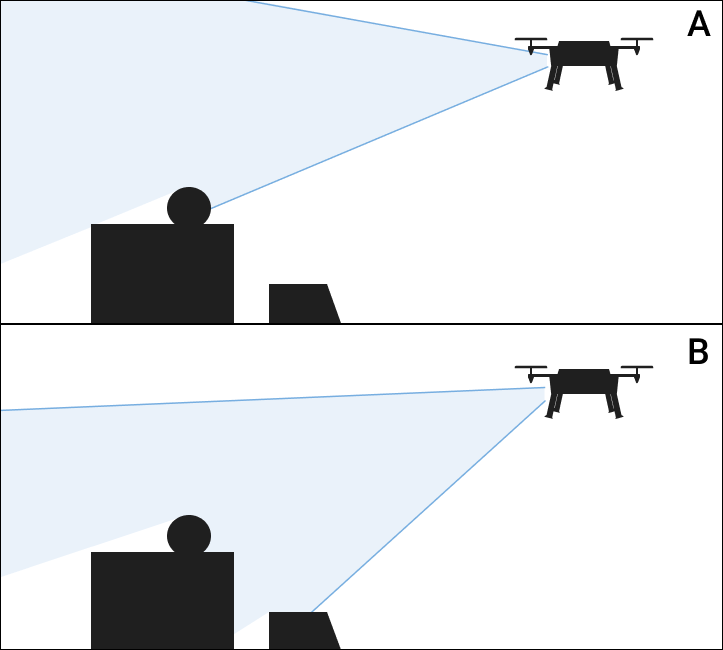
\includegraphics[width=0.7\linewidth]{img/FieldOfView}
	\caption{Depiction of the FOV for cameras mounted at different angles on a drone.\newline A: camera mounted vertically, B: camera mounted with a downward pointing angle.}
	\label{fig:custom_parts_FOV}
\end{figure}

Using zip ties results in the camera being mounted parallel to the ground. This leads to overlooking obstacles located below the field of view. This can be seen in figure 11.1 A. Adjusting the angle to be able to see as much as needed directly in front of the drone an the larger portion whats below the drone. Having the ability to capture obstacles directly in front of the drone is necessary, when wanting to be able to successfully let the drone navigate an environment autonomously. Therefor is a zip-tie solution valid, but far from optimal. A result of having a camera mounted parallel to the ground is the need to hover at a closer distance to the ground, which is potentially dangerous considering that in autumn we are not able to capture obstacles directly below the drone.

The second problem that arises when not using a mount fitted for use with, in case of autumn the ZED2i, is that the camera is not perfectly leveled. This portraits a major flaw when using a uneven camera together with a slam algorithm. Slam uses odometry data for localization and alignment of the ground plane. If the camera is slightly tilted when starting the algorithm and without manual adjustment the ground plane is going to be offset on one or multiple rotational axis. This results in the 3D model being a incorrect representation of reality. This phenomenon can be observed in Figure 11.2.

\begin{figure}[h]
	\centering
	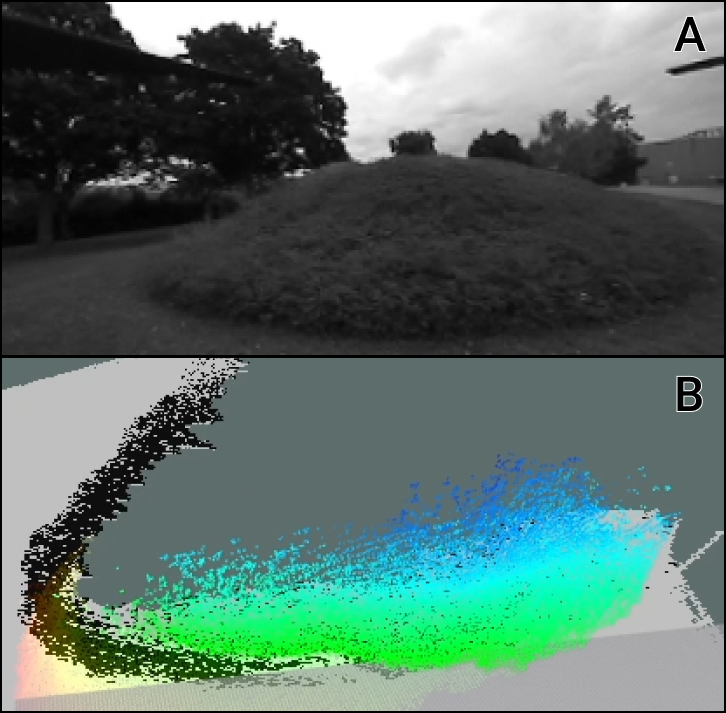
\includegraphics[width=0.5\linewidth]{img/MisalignedOdom}
	\caption{Resulting point cloud of unleveled camera with invalid odometry start data.\newline A: real life footage of the obstacle, B: tilted scan of the obstacle}
	\label{fig:custom_parts_misalignedOdom}
\end{figure}

\subsubsection{Design Process}

The solution to the aforementioned problems being a mount securing the ZED2i to the Matrice 100. Additionally to the specific characteristics the mount has to fulfill, the ZED2i is the newest model with commercial products like mounts not being available. Therefor, to attain this custom mount design and manufacturing methods have to be used. 
The design portion is done with the help of a CAD Software. CAD standing for Computer Aided Design, meaning that rather complex designs can be realized in a short amount of time and less effort than doing it the traditional way. The software used in the autumn project is Fusion360, due to its option for a free license and previously acquired knowledge working with this software. 
The mount had to perfectly fit the camera to ensure the safety of camera and drone. Therefor it is necessary to take measurements, which then are used to shape the design of the 3D-model. In Fusion360 this can be best realized using parameterized design. 

\begin{figure}[h]
	\centering
	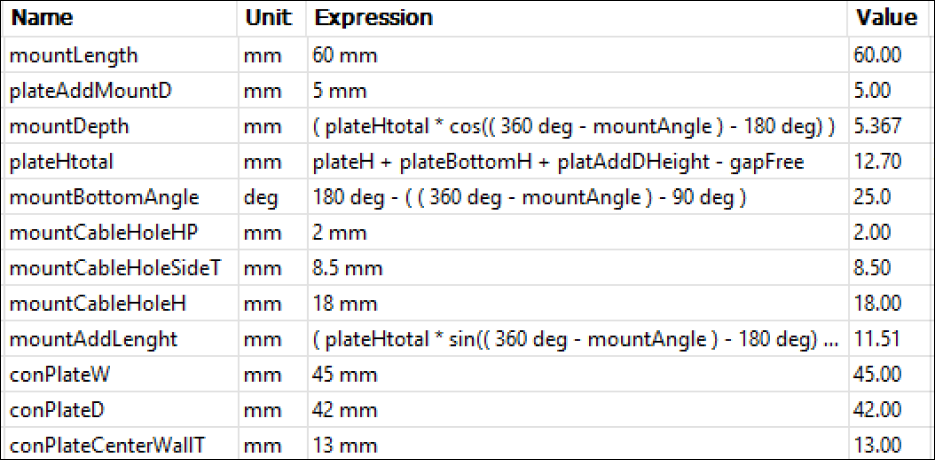
\includegraphics[width=0.7\linewidth]{img/Parameter}
	\caption{Excerpt of parameters used for the autumn camera mount design}
	\label{fig:custom_parts_parameter}
\end{figure}

Figure 11.3 depicts this concept of making the design dependent on parameters which can be easily adjusted. This allows for corrections to be made after the design processed is finished. Without linking sketches to parameters alterations would be time consuming and would result in an model clouded with sketches overriding previous adjustments. Furthermore changes affecting complex areas in the part lead to artifacts, which when removed take more time than redesigning the part in when applied to simple, one component models, like the mount in autumn. An important property in case of the autumn camera mount is the angle of the camera relative to the drone. This design principle makes it possible that changing the angle only means changing a number in a text-field, which implies the change of a number of different dimensions of the part. 
Fusion 360 additionally comes with the capability of rendering the resulting model, in order to get a feel for how it would look in physical form.

\begin{figure}[h]
	\centering
	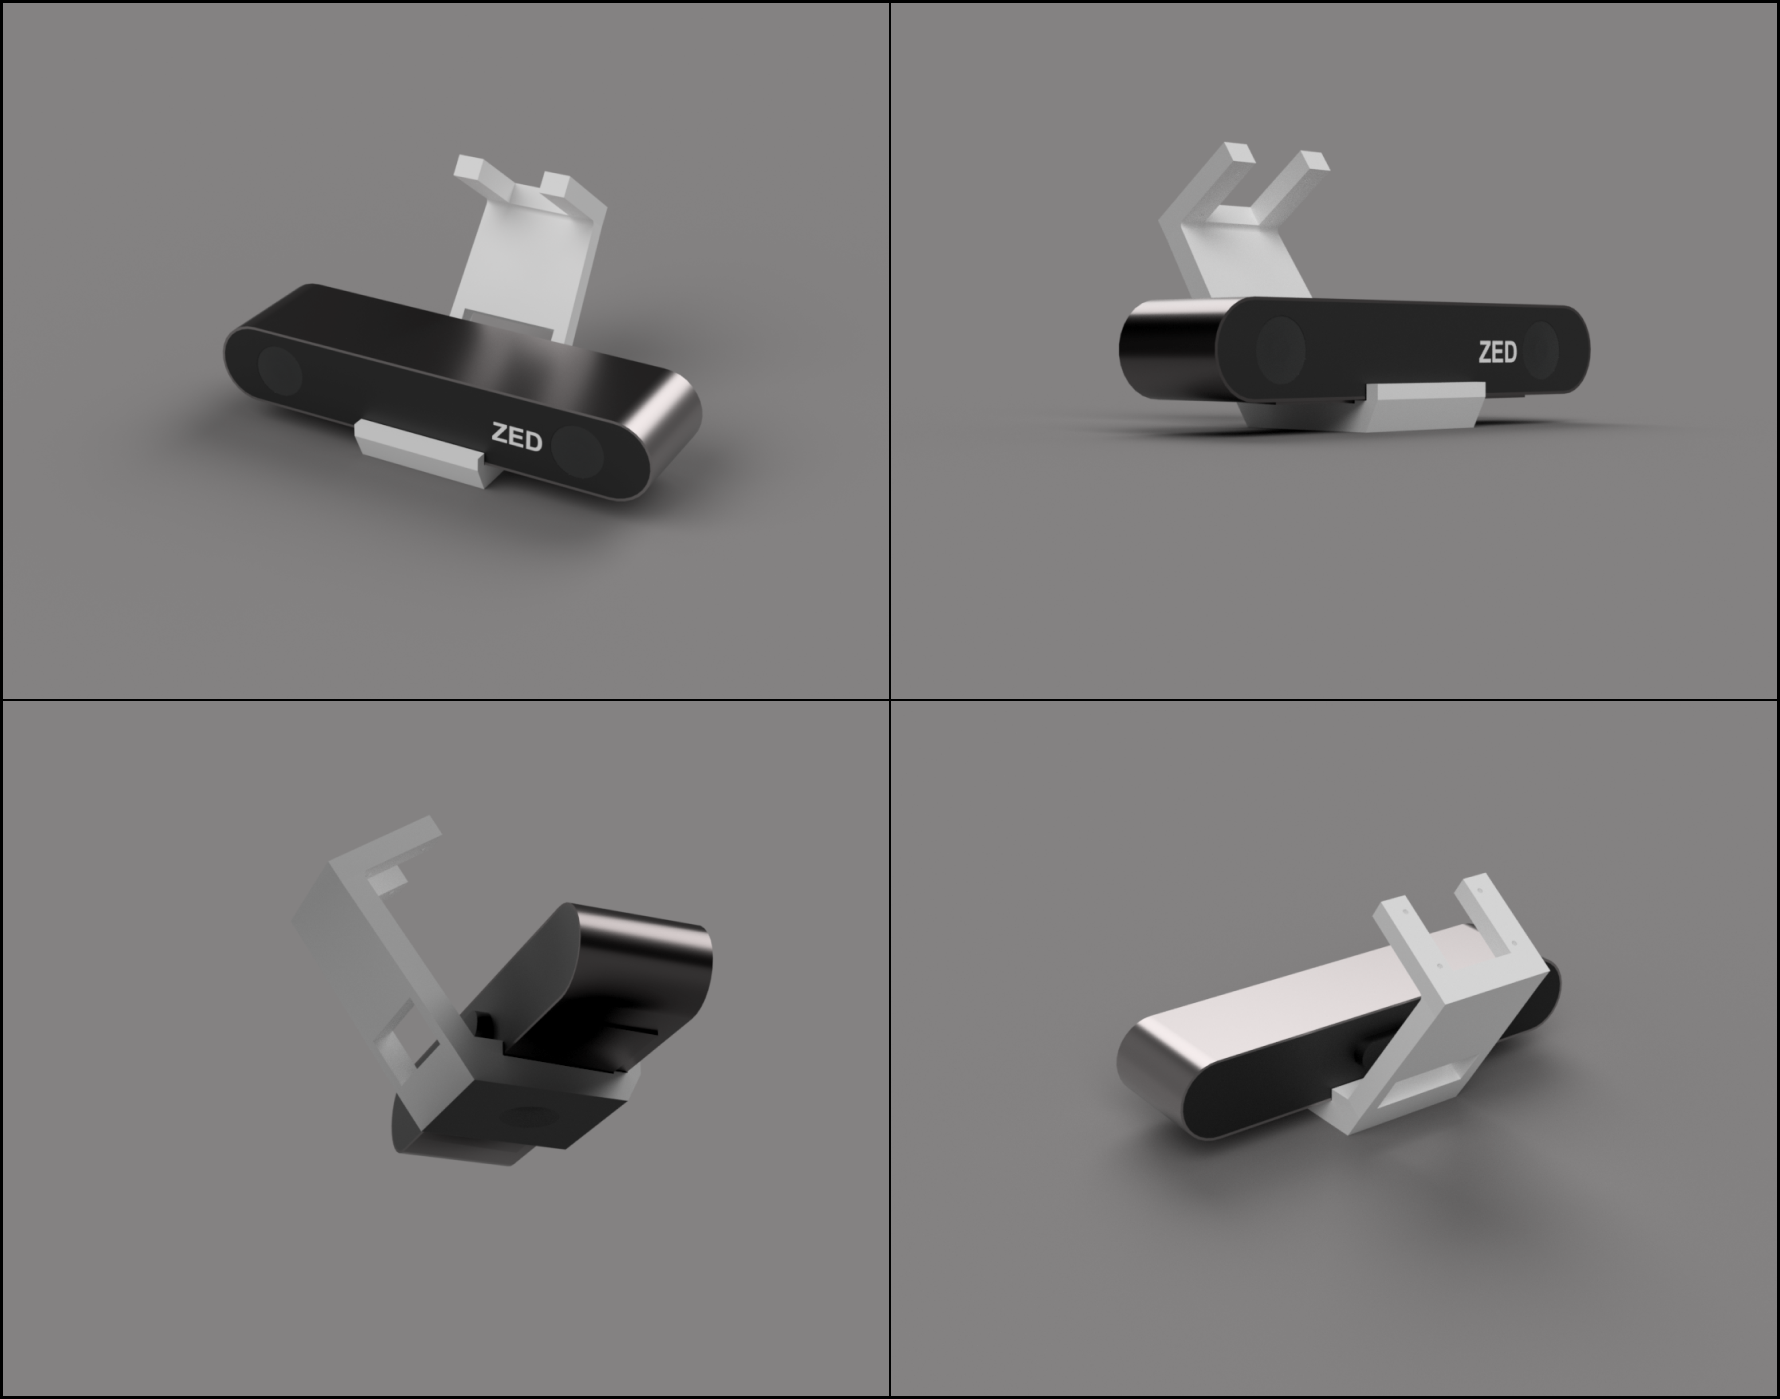
\includegraphics[width=0.6\linewidth]{img/MountRender}
	\caption{Render of the 3D-model for the camera mount attaching the ZED2i, also modeled and visible in the render, to the Matrice 100.}
	\label{fig:custom_parts_mountRender}
\end{figure}

\subsubsection{Manufacturing}

For the purpose of converting the 3D-model to an physical object, the simplest and most time efficient method is to utilize 3D-printing. Nowadays 3D-printing is a wide spread technique to make ideas reality with little time and money. Therefor it is an optimal solution for the autumn project. 
When going from a 3D-modeled design to an 3D-print a slicer is needed to convert the 3D-object to code the printer understands. With most 3D-printers printing in 2.5 dimensions, meaning that only the x and y axis move freely while the z only adjusts its height once a layer is finished. This principle is reflected in the resulting file once a 3D-model is sliced. The gcode consits of an header, defining settings for the print and a sequence of lines following it. A line of this gcode file would look like this: 
\[G1\ X120.95\ Y101.653\ E1.17355\]
The first part consisting of the identifier $G$ and a number, marks which command should be executed. In case of $G1$ it's "move in a straight line". Following the command specifier are parameters, for this example the x and y end position is needed to draw a line. Additionally marked with the identifier $E$, is the flow rate defining how much filament is going to be extruded when moving to the given position.

The final step to attaining the physical form of a gcode file, is printing it using a suitable 3D-printer. Autumn uses an Creality Ender 5, because of it's readability and print quality. Furthermore the choice of the correct filament for an successful 3D-print is needed. For a part, like the camera mount, which isn't under big stresses and no large forces are applied to it, filament like acrylonitrile butadiene styrene, commonly known as ABS, isn't needed. Therefor the most widely used filament, polylactide is most fitted for this print.

\begin{figure}[h]
	\centering
	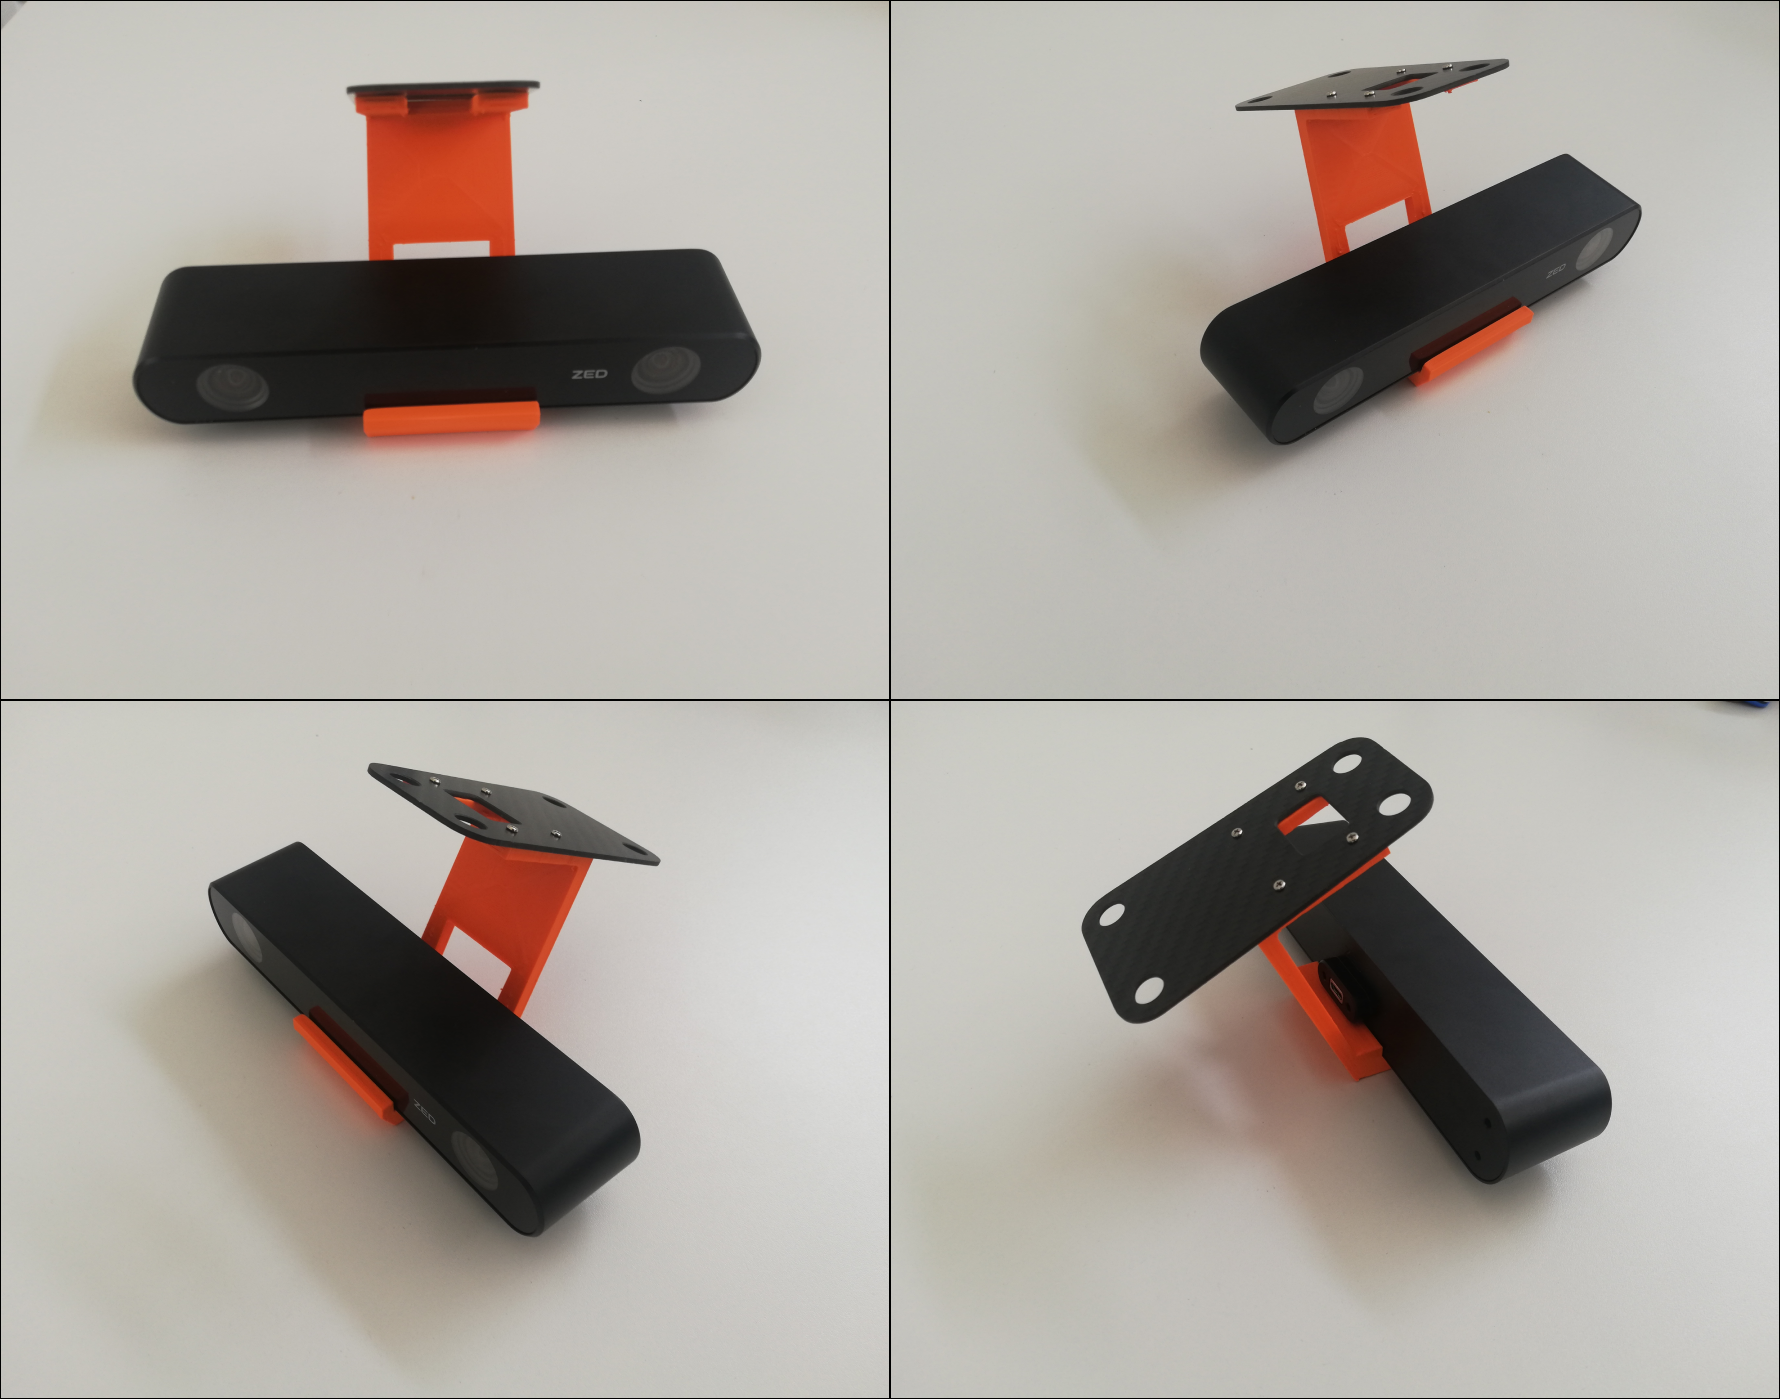
\includegraphics[width=0.6\linewidth]{img/MountPrint}
	\caption{3D-printed camera mount for the purpose of attaching the ZED2i to the Matrice 100. On top of the mount is the connection plate attaching on the drone.}
	\label{fig:custom_parts_mountPrint}
\end{figure}

\section{CAD Software}

This section is going to cover widespread CAD software solution. Nowadays computer aided design is a imperative principle, used in a variety of industries. CAD software improves the efficiency and quality of the design workflow. With free solutions being available, this industry standard has expanded to a clientele reaching from the leading companies to hobbyist creating innovation of the future in the comfort of their homes. Therefor when choosing an apt software, a multiplicity of properties have to be considered.

\subsection{SolidWorks}

SolidWorks being the industry leading CAD solution, it is hard to overlook in a comparison. SolidWorks offers a fast array of functionality for not only CAD, additionally it offers capabilities for computer aided manufacturing. 
The target audience for SolidWorks being experts in the field of modeling and design. Hereby is not only the UI designed to cater more to a clientele which is firm in their understanding of the computer aided design process, but also it offer more in-depth functionalities such as dynamic loading, linear and non-linear analysis and composite materials.\footcite{all3dpSolidWorksVsFusion2021}

\begin{figure}[h]
	\centering
	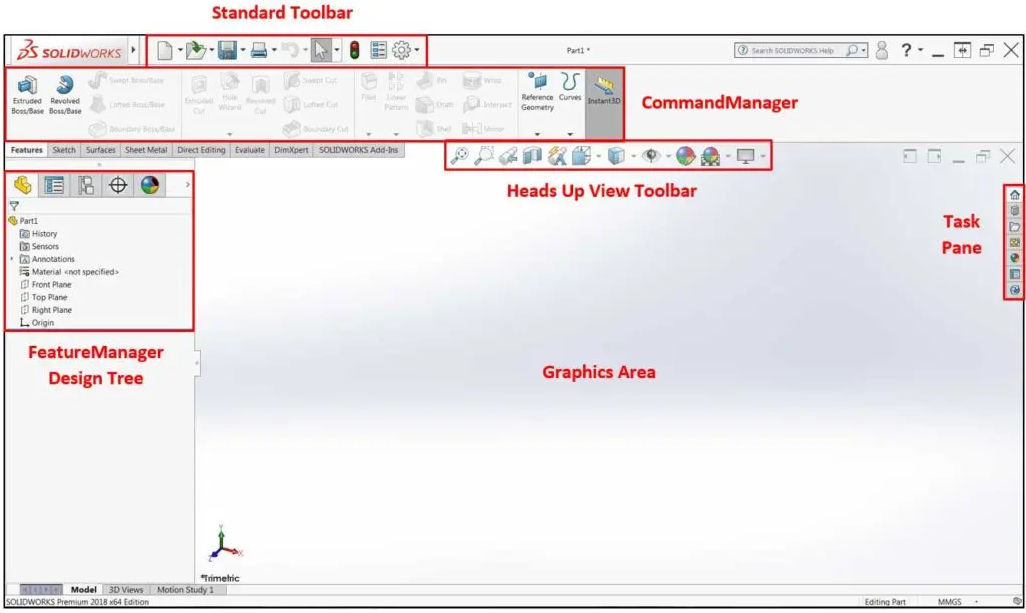
\includegraphics[width=0.6\linewidth]{img/SolidWorksUI}
	\caption{SolidWorks user interface broken up into its different components.\footcite{hawkridgesysUIBSolidWorks2019}}
	\label{fig:custom_parts_solidworks}
\end{figure}


\subsection{Fusion 360}

With Fusion 360 offering a non-commercial, free license option with limited functionality, it is wide spread amongst hobbiest and with its beginner friendly ui design and possibility for an educational license with the majority of the functional scope of the professional license. Features included in the professional subscription that are excluded otherwise are mostly cloud processing options and load and stress simulations.

\begin{table}
	\centering
	\begin{tabular}{ |p{3cm}||p{6cm}|p{3cm}|  }
		\hline
		\multicolumn{3}{|c|}{Fusion 360 Licenses} \\
		\hline
		License & Features & Price\\
		\hline
		Fusion 360 for personal use& Standard design and 3D modeling tools& free\\
		\hline
		Fusion 360& Standard design and 3D modeling tools, plus a fully featured CAM, CAE, and PCB development platform& 495\$ p.a.\\
		\hline
	\end{tabular}
	\caption{An overview of Fusion 360 licenses with their respective capabilities and prices.\footcite{autodeskFusionPersonalNoDate}}
\end{table}

\subsection{Autumn choice}

When comparing the two CAD solution, that are possibilities to be used in the autumn project, the most important characteristic is the user friendliness in respect to the state of knowledge the user already has. Both SolidWorks and Fusion 360 offer more than enough functionality to fulfill the needs of autumn. When looking at the monetary dimension, where for the needed functionality Fusion has no competition with its free license for personal use. Furthermore is the Fusion 360 workflow tailored to simple application, with a small amount of components. SolidWorks follows a assembly based principle, in contrast Fusion 360 is based on a multi-component architecture.\newline
In conclusion due to the limited amount of functionality required from a CAD software in the autumn project, Fusion 360 is being used.

\section{Manufacturing Process}

This section is going to focus on manufacturing methods available in the autumn project and compare them. Nowadays easy and fast prototyping is made possible with use of 3D-printing technology. 3D-Printing has evolved over the years, away from a science fiction concept, to an widely used tool in part manufacturing, filling the gap left open by the geometrical limitations of conventional methods.

\subsection{3D-Printing}

Autumn having an area of competence, split between skills when working with soft- and hardware, it is important to have the means to manufacture custom parts, tailored to the needs of the project. With 3D-Printing being an affordable and accurate technology, in terms of translating virtual concepts to physical object, it is an obvious choice to use for autumn.
When considering using 3D-printing in any kind of project, it is important to think about which method is best fitted for the application.

\subsubsection{FDM-Printing}

Fused Deposition Modeling is the conventional method of 3d-printing. FDM-Printing is characterized by the use of a filament, which is extruded, in order to build up the model layer by layer. The print-head consisting of an extruder, hot-end and nozzle, is moved in the x and y . Filament is fed to the hot-end via the extruder, where it is heated to its melting point and pushed through a nozzle which specifies the flow rate by constricting the flow. 
This simple approach enables an easy and fast realization of concepts and ideas. 
Drawbacks of this methods consist of decreased structural integrity in the z-direction of the print. 

\subsubsection{SLA-Printing}
